\documentclass[../main.tex]{subfiles}
\addbibresource{../bibfile.bib}

\begin{document}

\chapter{Analisi implementate}
In questo capitolo, verranno descritte nel dettaglio le tecniche di ricerca automatica delle vulnerabilità rese disponibili dalla piattaforma.
In particolare, verranno illustrate quali metodologie di analisi ogni tecnica utilizza e come esse concorrono al rilevamento
di particolari classi di vulnerabilità.
\section{VulnDetect}
Le tecniche che si basano sull'esecuzione simbolica devono tenere conto del problema noto con il nome di \textit{path explosion}: l'incremento delle
dimensioni di un programma porta ad un aumento esponenziale dei cammini praticabili presenti sul suo CFG, i quali possono crescere fino a diventare
potenzialmente infiniti se il programma contiene cicli non vincolati da una condizione di terminazione \cite{SE_Path_explosion}. 
Per evitare questo problema, l'esecutore simbolico può essere guidato in modo tale che esplori solamente una parte del CFG del programma, in modo tale da evitare che esso
esplori cammini potenzialmente inutili alla ricerca di vulnerabilità. \textbf{VulnDetect} \cite{VulnDetect} è una tecnica di ricerca per basata su esecuzione simbolica per la ricerca
di vulnerabilità di tipo \textbf{stack-based buffer-overflow}. L'implementazione di VulnDetect si basa sulle funzionalità offerte dalla piattaforma \textit{angr}.
Per evitare il problema della \textit{path explosion}, VulnDetect utilizza un'insieme di metodologie di analisi statica per guidare
l'esecutore simbolico ad analizzare solo i cammini potenzialmente vulnerabili del programma.
\subsection{Buffer overflow e Stack-Based Buffer Overflow}
Una delle classi di vulnerabilità software più diffuse nel panorama software moderno è quella che prende il nome di \textbf{buffer overflow} (CWE-120).
Questo tipo di vulnerabilità si presenta quando non avviene nessun controllo sulla lunghezza massima dei dati che devono essere salvati all'interno
di un buffer allocato in memoria. Il dato, quindi, può potenzialmente andare a sovrascrivere i dati posti in sezioni di memoria adiacenti all'area di allocazione
del buffer, potenzialmente quindi andando a sovrascrivere dati fondamentali per la corretta esecuzione del programma. 
Questa problematica è particolarmente rilevante nei linguaggi non \textit{memory safe}, dove il compito di gestione della memoria del programma è affidato
al programmatore. Quando il buffer-overflow può avvenire su un buffer allocato nello stack del programma, la vulnerabilità prende il nome di \textbf{stack-based buffer overflow} (CWE-121).
La presenza di questo tipo di vulnerabilità può portare a conseguenze catastrofiche: un attaccante, per esempio, potrebbe sovrascrivere l'indirizzo di ritorno della funzione in cui viene dichiarato il buffer, 
potenzialmente portando il programma ad eseguire codice malevolo presente nell'input (shellcode).
\subsection{Strategia di analisi}
VulnDetect struttura la strategia di analisi in due fasi distinte:
\begin{enumerate}
    \item \textbf{Analisi statica}: Le vulnerabilità di tipo \textit{buffer overflow} sono principalmente causate dall'utilizzo improprio di funzioni pericolose (in C, per esempio \textit{gets, scanf,}...) e dalla mancanza di controlli
    sulla lunghezza dell'input dell'utente. Per migliorare l'efficienza dell'esecuzione simbolica, VulnDetect applica una sequenza di tecniche di analisi statica sul programma:
    \begin{enumerate}
        \item \textbf{Identificazione di operazione sensibili}: Innanzitutto, viene caricato il programma tramite la classe \textit{Project} di angr.
        Successivamente, si procede al recupero degli indirizzi delle funzioni di libreria potenzialmente pericolose, accedendo alle informazioni contenute nella \textit{Procedure Linkage Table} (PLT).
        Per determinare quali funzioni recuperare dalla PLT, il programma di analisi mantiene al suo interno una \textbf{lista di nomi di funzioni potenzialmente pericolose}.
        Viene infine recuperato, sempre tramite angr, il CFG del programma, il quale viene attraversato in modo tale da individuare \textbf{gli indirizzi nel programma in cui avvengono chiamate a funzioni pericolose}.
        \item \textbf{Program slicing}: Per prima cosa, viene creato il Data Dependency Graph del programma. Dopodiché, viene effettuato \textit{program slicing} per ogni indirizzo di chiamata a funzione pericolosa individuato nel passo precedente, in modo tale
        da estrarre i segmenti di codice correlati ad ogni chiamata. Chiameremo questi segmenti \textit{hotspot code segments}.
    \end{enumerate}
    \item \textbf{Vulnerability detection}: La ricerca di vulnerabilità viene effettuata eseguendo simbolicamente il programma, simulando l'input dell'utente con un \textbf{input simbolico}. Per evitare \textit{path explosion}, l'esecutore simbolico viene guidato durante il processo di esecuzione usando gli \textit{hotspot code segments} ottenuti
    durante la fase di analisi statica. Così facendo, l'esecuzione simbolica esplorerà solamente i cammini legati alla ricerca della vulnerabilità, invece di tutti i cammini praticabili del CFG. Quando l'esecuzione arriva ad un punto del programma dove avviene una chiamata ad una funzione pericolosa, è necessario 
    continuare da quel punto l'esecuzione simbolica del programma per assicurarsi che l'operazione che svolge porti ad una vulnerabilità. In caso di presenza di buffer overflow, il registro \textit{EIP} (Extended Instruction Pointer) conterrà un valore simbolico. Questo stato non permette quindi all'esecutore di determinare quale sarà il prossimo
    stato in cui si troverà il programma e quindi l'esecuzione viene interrotta. In angr, questo tipo di stati del programma prendono il nome di \textbf{unconstrained states}. 
    Sarà quindi presente nel programma una vulnerabilità di tipo \textit{stack-based buffer overflow} se l'esecutore simbolico trova almeno uno stato \textit{unconstrained} durante l'esecuzione.
\end{enumerate}
\begin{figure}[H]
    \centering
    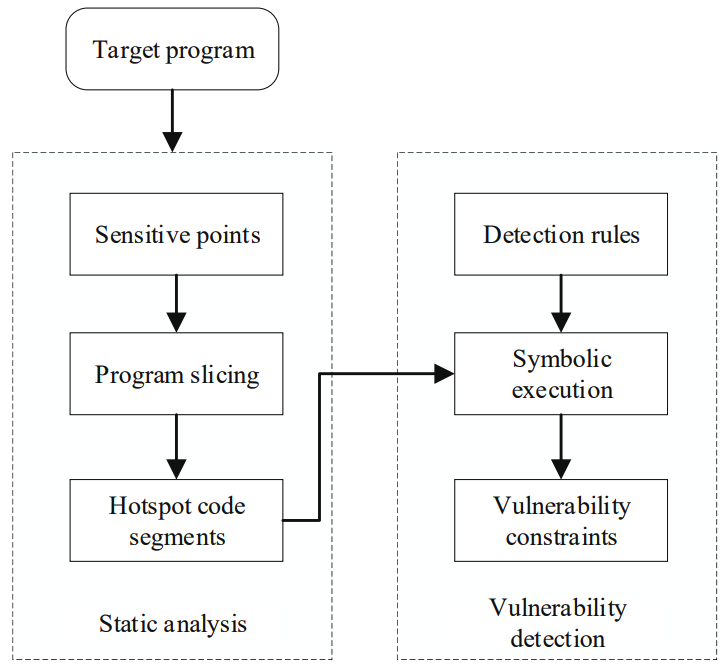
\includegraphics[width = 0.60\textwidth]{../images/VulnDetect.png}
    \caption{Processo di analisi impiegato da VulnDetect. Immagine proveniente da \cite{VulnDetect}}
\end{figure}
\section{Arbiter}








\end{document}





